\documentclass[uplatex,dvipdfmx,11pt,a4paper]{jsarticle}

\usepackage[a4paper,margin=24mm]{geometry}
\usepackage[dvipdfmx]{graphicx}
\usepackage{booktabs}
\usepackage{longtable}
\usepackage{caption}
\usepackage{float}
\usepackage{xcolor}
\usepackage[dvipdfmx]{hyperref}
\usepackage{pxjahyper}

\hypersetup{
  colorlinks=true,
  linkcolor=blue,
  urlcolor=blue,
  citecolor=blue
}

\captionsetup{font=small,labelfont=bf}
\renewcommand{\figurename}{図}
\renewcommand{\tablename}{表}
\renewcommand{\refname}{参考文献}
\renewcommand{\abstractname}{要旨}

\title{意味埋め込みを用いた仏教文献の宗派的配置・訳者差・多言語対応の予備的検討}
\author{未定}
\date{2026年6月1日}

\begin{document}

\maketitle

\begin{abstract}
本稿は、漢訳仏典および日本撰述仏教文献を対象に、意味埋め込みによって宗派別の参照テキスト群を可視化できるかを検討する予備的研究である。対象には、浄土系、法華系、真言系、禅系、華厳系、法相系に関係する15テキストを用いた。各本文をチャンク化し、\texttt{text-embedding-3-large} によってチャンク埋め込みを作成し、本文単位のベクトルはチャンクベクトルの平均として得た。さらに、宗派重心と訳者重心を計算し、平均点の2次元配置、チャンク分布、類似度ヒートマップ、近傍テキストを確認した。加えて、漢訳『解深密経』とチベット大蔵経由来の84000英訳を用い、言語を越えて同一経典性が近傍関係として現れるかを小規模に検証した。

結果として、阿弥陀経とその玄奘訳別訳である『稱讃淨土佛攝受經』は、訳者が異なるにもかかわらず高い類似度を示した。一方で、玄奘訳の複数テキストは、訳者のみを理由に強くまとまるわけではなかった。チャンク分布では、本文平均点だけでは見えにくい各経典内部の広がりと重なりが確認でき、とくに阿弥陀経二訳はチャンク近傍混合率が高かった。これは、意味埋め込みが主として内容・主題の近さを捉え、訳語選択や文体上の癖は別の特徴量として扱う必要があることを示唆する。さらに親鸞文献側の小実験では、『入出二門偈』に玄奘訳『称讃浄土経』の明示的参照が確認され、『教行信証』では阿弥陀経二訳のどちらか一方だけに還元しにくい重層的な近さが見られた。また、浄土三部経や真言系密教経典には一定のまとまりが見られたが、禅系については経典のみでは宗派差を十分に表現できなかった。多言語パイロットでは、84000英訳 \textit{The Teaching Explaining the Thought} の最近傍が漢訳『解深密経』となり、少なくともこの組み合わせでは意味埋め込みが言語差を越えて同一経典性を捉えうることが示された。
\end{abstract}

\noindent\textbf{キーワード:} 漢訳仏典、宗派比較、意味埋め込み、阿弥陀経、玄奘、鳩摩羅什、多言語比較、仏教文献情報学

\section{はじめに}

日本仏教の各宗派は、それぞれ特定の経典、祖師文献、儀礼的読誦テキストを重視してきた。たとえば浄土系では浄土三部経および祖師文献が重要であり、真言宗では大日経、金剛頂経、理趣経などの密教経典が中心的な位置を占める。一方、禅宗では般若心経、金剛経、維摩経などが参照されるが、宗派的特徴は経典そのものよりも語録、清規、祖師文献に強く現れる可能性がある。

近年の大規模言語モデルおよび埋め込みモデルは、テキストの意味的近さを高次元ベクトルとして表現できる。本研究では、この手法を仏教文献に適用し、宗派ごとの参照テキスト群の配置を可視化できるかを検討する。あわせて、阿弥陀経の異訳や同一訳者の複数テキストを用い、意味的近さと翻訳文体の差がどのように現れるかを予備的に確認する。さらに、漢訳仏典とチベット大蔵経由来の英訳を対照し、意味埋め込みが言語を越えた同一経典性をどの程度拾えるかを試験的に確認する。

本稿の目的は、宗派分類の正解モデルを作ることではない。むしろ、各宗派が参照するテキスト群を意味空間上に置いたとき、どのような近接関係や解釈上の問題が現れるかを把握することである。

\section{研究課題}

本稿では、以下の四つの問いを設定する。

\begin{enumerate}
  \item 意味埋め込みによって、浄土三部経や真言系密教経典のような主題的まとまりを確認できるか。
  \item 宗派ごとの参照テキスト群を重心として可視化した場合、宗派の特徴をどの程度表現できるか。
  \item 阿弥陀経の異訳および同一訳者の複数テキストを比較したとき、意味の近さと翻訳文体の差を区別できるか。
  \item 漢訳仏典とチベット大蔵経由来の英訳を比較したとき、同一経典性は言語差を越えて近傍関係として現れるか。
\end{enumerate}

\section{データ}

本文は主にSAT大正新脩大藏經テキストデータベースから取得した。『顯淨土眞實教行證文類』については、浄土真宗本願寺派総合研究所『浄土真宗聖典』聖教データベースの収載・利用規定を確認し、同データベースを利用した旨を明記する必要があるため、本稿の参考文献にも同データベースを掲げる。一部の検証用テキストには、全文ではない既存取得本文を用いた。v0.1で用いたテキスト数は15、チャンク数は433である。多言語パイロットでは、SAT由来の漢訳『解深密経』と、84000 Reading Roomで公開されている \textit{The Teaching Explaining the Thought}（Toh 106）英訳を用いた。84000本文は研究用キャッシュとして扱い、本文そのものは本稿に転載しない。

親鸞文献における阿弥陀経二訳の参照分析では、上記コーパスとは別に、真宗聖典検索サイト所収の『入出二門偈』該当頁も参照した。この追加資料は宗派別マップ全体の平均ベクトルには組み込まず、経名・訳者名の明示、訳語・句の指標、ならびに『教行信証』チャンクと阿弥陀経二訳チャンクの近傍関係を確認するために用いた。

\begin{longtable}{llll}
\caption{対象テキスト}\\
\toprule
系統 & テキスト & ID & 訳者・著者 \\
\midrule
\endfirsthead
\toprule
系統 & テキスト & ID & 訳者・著者 \\
\midrule
\endhead
浄土系 & 佛説無量壽經 & T0360 & 康僧鎧 \\
浄土系 & 佛説觀無量壽佛經 & T0365 & 畺良耶舍 \\
浄土系 & 佛説阿彌陀經 & T0366 & 鳩摩羅什 \\
浄土系 & 稱讃淨土佛攝受經 & T0367 & 玄奘 \\
浄土真宗 & 顯淨土眞實教行證文類 & J-SOKEN聖教DB & 親鸞 \\
法華系 & 妙法蓮華經 & T0262 & 鳩摩羅什 \\
法華・禅系 & 觀世音菩薩普門品 & T0262 & 鳩摩羅什 \\
真言系 & 大毘盧遮那成佛神變加持經 & T0848 & 善無畏・一行 \\
真言系 & 金剛頂一切如來眞實攝大乘現證大教王經 & T0865 & 不空 \\
真言系 & 大樂金剛不空眞實三麼耶經 & T0243 & 不空 \\
禅・真言系 & 般若波羅蜜多心經 & T0251 & 玄奘 \\
法相系 & 解深密經 & T0676 & 玄奘 \\
禅系 & 金剛般若波羅蜜經 & T0235 & 鳩摩羅什 \\
禅系 & 維摩詰所説經 & T0475 & 鳩摩羅什 \\
華厳系 & 大方廣佛華嚴經 & T0279 & 實叉難陀 \\
\bottomrule
\end{longtable}

本実験は予備的なものであり、すべての大部経典を完全な全文として取得できているわけではない。特に法華経の既存取得本文は短く、全文ではない可能性が高い。また、SAT本文の再配布ではなく、実験結果の要約と派生データの確認を目的とする。

\section{方法}

\subsection{チャンク化と埋め込み}

本文は既定で700トークン、100トークンの重なりによりチャンク化した。各チャンクに対して \texttt{text-embedding-3-large} による埋め込みを作成した。同一モデル・同一本文のチャンクについてはキャッシュを利用し、再実行時にAPIを呼び直さないようにした。本文単位のベクトルは、当該本文に属するチャンクベクトルの平均として計算した。

\subsection{類似度と重心}

本文間の類似度はコサイン類似度によって計算した。宗派重心は、当該宗派に属する \texttt{core\_sutra} および \texttt{founder\_text} の本文ベクトルの平均として定義した。訳者重心は、同一訳者に属する複数テキストの本文ベクトルの平均として定義した。ただし、今回の訳者重心はサンプル数が少ないため、可視化上の補助線として扱う。

\subsection{可視化と対照実験}

本文ベクトル、宗派重心、訳者重心を同一空間に配置し、2次元表示にはPCAを用いた。阿弥陀経二訳については、意味埋め込みに加えて文字単位TF-IDFも計算した。文字単位TF-IDFでは2から5文字のn-gramを用いた。これは、意味的近さではなく、語彙選択や表記の差を捉えるための簡易的な対照実験である。

平均ベクトルだけでは、長い経典や複数主題を含む文献の内部的な広がりが見えなくなる。そこで、主要テキストについてはチャンク単位の埋め込みをPCAで2次元表示し、各テキストのチャンク群に対して1標準偏差楕円を重ねた。また、2次元投影の重なりは歪みを含むため、元の高次元埋め込み空間で、あるテキストのチャンクのtop-5近傍に相手テキストのチャンクがどの程度入るかを「チャンク近傍混合率」として計算した。

\subsection{多言語パイロット}

多言語比較では、84000 Reading Room の \textit{The Teaching Explaining the Thought}（Toh 106）をHTMLから抽出し、SAT由来の漢訳『解深密経』（T0676）と比較した。対照群として、金剛経、維摩経、般若心経、阿弥陀経の漢訳を加えた。評価は、84000英訳の本文ベクトルから見た漢訳テキストの最近傍順位によって行った。

\section{結果}

\subsection{宗派別お経マップ}

図\ref{fig:semantic-map}に、本文ベクトルおよび訳者重心をPCAで2次元表示した結果を示す。浄土系テキストは左上方向に比較的近く配置され、真言系密教経典は下方向にまとまる傾向が見られる。一方、禅系の経典のみからは、曹洞宗・臨済宗・黄檗宗の差は明確には出なかった。

\begin{figure}[H]
  \centering
  
\includegraphics[width=\linewidth]{../figures/sect-sutra-semantic-map.png}
  \caption{意味埋め込みによる宗派別お経マップ。丸は本文、菱形は訳者重心を表す。}
  \label{fig:semantic-map}
\end{figure}

\subsection{チャンク分布と広がり}

図\ref{fig:chunk-overview}は、本文平均点ではなく、各本文を構成するチャンク群を点として表示したものである。楕円は各テキストの1標準偏差範囲を表す。平均点マップでは一点に集約されるテキストも、チャンク単位では主題の広がりや他テキストとの部分的重なりを持つことが分かる。特に、教行信証は引用や教義的総合を含むため、チャンク分布の広がりが大きい。

\begin{figure}[H]
  \centering
  
\includegraphics[width=\linewidth]{../figures/sect-sutra-chunk-distribution-overview.png}
  \caption{主要テキストのチャンク分布と1標準偏差楕円。小点はチャンク、濃い丸は各テキストのチャンク重心を表す。}
  \label{fig:chunk-overview}
\end{figure}

図\ref{fig:chunk-focus}は、代表的な組み合わせを局所的にPCA表示したものである。阿弥陀経二訳では、平均点だけでなくチャンク分布にも重なりが見られる。一方、真言系密教経典や般若・法相・禅系対照では、平均点の近さと分布の形が一致しない場合があり、本文全体を一点に潰すことの情報損失が確認できる。

\begin{figure}[H]
  \centering
  
\includegraphics[width=\linewidth]{../figures/sect-sutra-chunk-distribution-focus.png}
  \caption{代表ペア・グループのチャンク分布。各パネル内でPCAを再計算し、局所的な重なりを見やすくしている。}
  \label{fig:chunk-focus}
\end{figure}

高次元空間で計算したチャンク近傍混合率を図\ref{fig:chunk-overlap}に示す。値が大きいほど、相手テキストのチャンクが近傍に混ざりやすい。阿弥陀経二訳は0.37と高く、異訳間で分布が混ざる傾向が確認できる。対照的に、阿弥陀経と理趣経のような主題差の大きい組み合わせでは混合率が低い。

\begin{figure}[H]
  \centering
  
\includegraphics[width=0.9\linewidth]{../figures/sect-sutra-chunk-overlap-heatmap.png}
  \caption{チャンク近傍混合率による分布重なり。各セルは、二つのテキストのチャンクを合わせたとき、各チャンクのtop-5近傍に相手テキストのチャンクが入る割合の平均を表す。}
  \label{fig:chunk-overlap}
\end{figure}

図\ref{fig:overlap-vs-centroid}は、本文平均ベクトルの類似度とチャンク近傍混合率を同時に見たものである。右上に位置する阿弥陀経二訳は、平均点も近く、チャンク分布も強く混ざっている。一方、教行信証と浄土三部経は本文平均ベクトルでは近いが、チャンク近傍混合率は低めである。これは、教行信証が三部経を根拠として強く参照しつつも、本文全体としては引用、注釈、教義的論述を含む大きな複合文献であり、全チャンクが三部経チャンクと一様に混ざるわけではないことを示す。

\begin{figure}[H]
  \centering
  
\includegraphics[width=0.9\linewidth]{../figures/sect-sutra-overlap-vs-centroid.png}
  \caption{本文平均ベクトルの類似度とチャンク近傍混合率の関係。右上ほど、本文平均点も近く、部分単位でも分布が混ざりやすい。}
  \label{fig:overlap-vs-centroid}
\end{figure}

表\ref{tab:bridge-chunks}に、代表的な組み合わせについて、最も近いチャンクペアを示す。本文の転載を避けるため、チャンクIDと類似度のみを示した。教行信証と三部経の組み合わせでは、橋渡しチャンクの類似度は0.71から0.80程度と高い。したがって、三部経との部分的対応は確かに現れているが、混合率は低く、教行信証全体が三部経そのものと同じ分布になるわけではない。

\begin{table}[H]
\centering
\small
\caption{代表ペアの橋渡しチャンク。KGSは教行信証を表す。}
\label{tab:bridge-chunks}
\begin{tabular}{llrrr}
\toprule
ペア & 最近接チャンクペア & チャンク類似度 & 本文類似度 & 混合率 \\
\midrule
阿弥陀/稱讃 & T0366 0005 / T0367 0010 & 0.7672 & 0.8825 & 0.3684 \\
教行/無量寿 & KGS 0002 / T0360 0004 & 0.7969 & 0.8797 & 0.0438 \\
教行/観無量寿 & KGS 0088 / T0365 0002 & 0.7095 & 0.8375 & 0.0127 \\
教行/阿弥陀 & KGS 0098 / T0366 0005 & 0.7250 & 0.8058 & 0.0147 \\
無量寿/観無量寿 & T0360 0021 / T0365 0008 & 0.7660 & 0.9102 & 0.1680 \\
金剛頂/理趣 & T0865 0000 / T0243 0000 & 0.8176 & 0.8405 & 0.1161 \\
金剛/維摩 & T0235 0004 / T0475 0022 & 0.7235 & 0.8770 & 0.1404 \\
阿弥陀/理趣 & T0366 0005 / T0243 0007 & 0.5900 & 0.6816 & 0.0375 \\
\bottomrule
\end{tabular}
\end{table}

主要テキスト間の類似度を図\ref{fig:heatmap}に示す。阿弥陀経、玄奘訳別訳、無量寿経、観無量寿経の近接が確認できる。また、大日経、金剛頂経、理趣経の間にも比較的高い類似度が見られる。

\begin{figure}[H]
  \centering
  
\includegraphics[width=0.92\linewidth]{../figures/sect-sutra-similarity-heatmap.png}
  \caption{主要テキスト間のコサイン類似度。値が大きいほど意味埋め込み上で近い。}
  \label{fig:heatmap}
\end{figure}

\subsection{阿弥陀経二訳}

鳩摩羅什訳『佛説阿彌陀經』と玄奘訳『稱讃淨土佛攝受經』を比較したところ、意味埋め込みでは高い類似度を示した。一方、文字単位TF-IDFでは低い類似度となった（図\ref{fig:amida-comparison}）。

\begin{figure}[H]
  \centering
  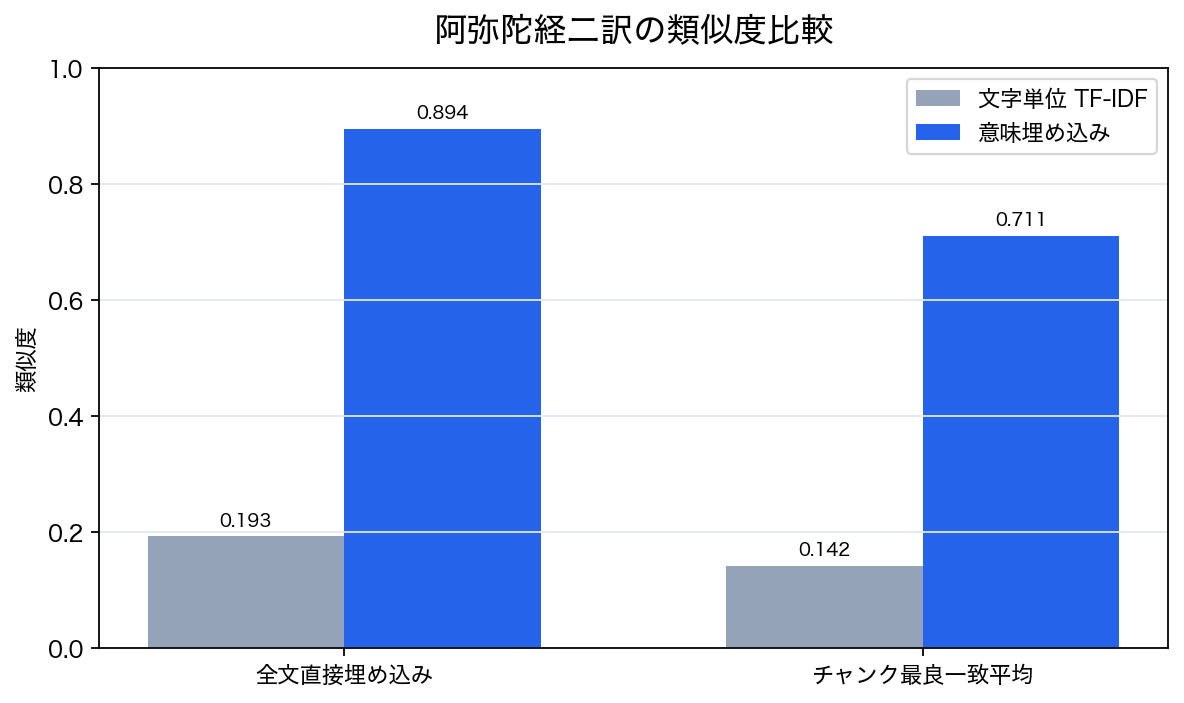
\includegraphics[width=0.78\linewidth]{../figures/amida-two-translation-comparison.png}
  \caption{阿弥陀経二訳の類似度比較。意味埋め込みは内容の近さを、文字単位TF-IDFは語彙・表記差を強く反映する。}
  \label{fig:amida-comparison}
\end{figure}

\begin{table}[H]
\centering
\caption{阿弥陀経から見た近傍テキスト}
\begin{tabular}{lr}
\toprule
近傍テキスト & コサイン類似度 \\
\midrule
稱讃淨土佛攝受經 & 0.8825 \\
無量寿経 & 0.8694 \\
観無量寿経 & 0.8446 \\
妙法蓮華経抜粋本文 & 0.8275 \\
教行信証 & 0.8058 \\
\bottomrule
\end{tabular}
\end{table}

\subsection{親鸞文献における阿弥陀経二訳}

親鸞が阿弥陀経をどの漢訳、あるいはどの注釈伝統を通して読んでいたかは、意味埋め込みだけで判定できる問題ではない。鳩摩羅什訳『佛説阿彌陀經』と玄奘訳『稱讃淨土佛攝受經』は原内容が近く、意味ベクトルでは強く近接する。そのため、本稿では追加の小実験として、証拠を三層に分けた。第一に、経名・訳者名の明示である。第二に、羅什訳または玄奘訳に寄りやすい訳語・句の指標である。第三に、『教行信証』チャンクが阿弥陀経二訳のどちらのチャンクへ近いかという意味近傍である。

図\ref{fig:shinran-source-markers}に、親鸞文献側のソース指標を示す。『入出二門偈』該当頁では、『称讃浄土経』と玄奘訳であることが明示され、玄奘訳側の讃嘆モチーフに対応する語句も検出された。一方、『教行信証』では、羅什訳側に寄る句と『称讃浄土経』の経名参照が併存する。したがって、『教行信証』については、単純に羅什訳または玄奘訳のどちらか一方に帰属させるより、三部経、異訳、法照・善導・元照などの注釈伝統が重なる文献として読む必要がある。

\begin{figure}[H]
  \centering
  
\includegraphics[width=0.86\linewidth]{../figures/shinran-amida-source-markers.png}
  \caption{親鸞文献側の阿弥陀経二訳ソース指標。経名・訳者名の明示と、訳語・句の指標を分けて表示した。}
  \label{fig:shinran-source-markers}
\end{figure}

『教行信証』本文平均ベクトルから見た類似度は、羅什訳『阿弥陀経』が0.8058、玄奘訳『稱讃淨土佛攝受經』が0.8152であった。玄奘訳の方がわずかに高いが、差は0.0094にすぎない。図\ref{fig:shinran-chunk-affinity}のチャンク単位の推移を見ても、二訳への近さは本文全体で交錯している。これは、親鸞文献の内部に、経文引用、釈義、祖師文献引用、教義的論述が混在していることを反映していると考えられる。

\begin{figure}[H]
  \centering
  
\includegraphics[width=0.95\linewidth]{../figures/shinran-kyogyoshinsho-amida-chunk-affinity.png}
  \caption{『教行信証』チャンクから見た阿弥陀経二訳への最大類似度。赤は玄奘訳、青は羅什訳への近さを表す。}
  \label{fig:shinran-chunk-affinity}
\end{figure}

\begin{table}[H]
\centering
\small
\caption{親鸞文献側から見た阿弥陀経二訳の証拠}
\label{tab:shinran-amida-source}
\begin{tabular}{p{0.17\linewidth}p{0.21\linewidth}p{0.22\linewidth}p{0.25\linewidth}}
\toprule
対象 & 羅什訳側 & 玄奘訳側 & 解釈 \\
\midrule
教行信証 & 固有句あり、チャンク最大0.7250 & 経名参照あり、本文平均0.8152 & 両訳・注釈伝統が重なる。単独決定は不可。 \\
入出二門偈 p543 & 目立たず & 称讃浄土経・玄奘訳を明示 & 玄奘訳参照の強い証拠。 \\
阿弥陀経集註 & 未投入 & 未投入 & 次段階の本命資料。経文・註記・裏書の分離が必要。 \\
\bottomrule
\end{tabular}
\end{table}

この小実験の要点は、阿弥陀経二訳の問題を「意味的にどちらに近いか」だけで解かないことである。意味埋め込みは、阿弥陀経二訳の同内容性をうまく捉える反面、訳語選択や引用経路の違いを薄める。親鸞文献のソース分析では、埋め込み近傍を探索の入口としつつ、経名・訳者名、固定句、注釈書の引文を別レイヤーとして重ねる必要がある。

\subsection{訳者重心}

訳者重心は、不空、玄奘、鳩摩羅什の3種を作成した。玄奘訳『稱讃淨土佛攝受經』の近傍は、同じ玄奘訳の般若心経や解深密経ではなく、鳩摩羅什訳『阿弥陀経』および浄土系経典であった。これは、今回の意味埋め込みでは、訳者差よりも主題・内容の影響が強いことを示唆する。

\begin{table}[H]
\centering
\caption{訳者重心の構成}
\begin{tabular}{lll}
\toprule
訳者 & テキスト数 & 対象 \\
\midrule
不空 & 2 & 金剛頂経、理趣経 \\
玄奘 & 3 & 稱讃淨土佛攝受經、般若心経、解深密経 \\
鳩摩羅什 & 5 & 阿弥陀経、法華経、観音経、金剛経、維摩経 \\
\bottomrule
\end{tabular}
\end{table}

\subsection{多言語比較パイロット}

84000英訳 \textit{The Teaching Explaining the Thought}（Toh 106）を問い合わせテキストとし、漢訳テキスト群とのコサイン類似度を比較した。表\ref{tab:multilingual-pilot}に上位近傍を示す。

\begin{table}[H]
\centering
\caption{84000英訳 Toh 106 から見た漢訳近傍}
\label{tab:multilingual-pilot}
\begin{tabular}{llr}
\toprule
順位 & 近傍テキスト & コサイン類似度 \\
\midrule
1 & 解深密經（T0676） & 0.7662 \\
2 & 維摩詰所説經（T0475） & 0.6926 \\
3 & 金剛般若波羅蜜經（T0235） & 0.6922 \\
4 & 般若波羅蜜多心經（T0251） & 0.6167 \\
5 & 佛説阿彌陀經（T0366） & 0.5683 \\
\bottomrule
\end{tabular}
\end{table}

結果として、84000英訳の最近傍は対応する漢訳『解深密経』となった。このことは、少なくとも本組み合わせでは、意味埋め込みが英訳と漢訳という言語差を越えて同一経典性を拾えている可能性を示す。ただし、維摩経や金剛経も0.69台で近く、大乗経典一般の主題的近さも反映されているため、同一経典判定として用いるには、異言語ペアをさらに増やし、同一作品内類似度と別作品類似度の差を検証する必要がある。

\section{考察}

阿弥陀経二訳の結果は、意味埋め込みが語彙差や訳語差を越えて、内容の近さを強く捉えることを示している。これは、同一または近接する原内容の漢訳を検出する用途には有用である可能性がある。一方で、文字単位TF-IDFでは阿弥陀経二訳の類似度が低く出た。これは、文体、訳語、語彙選択、固有名詞表記の差が文字n-gram特徴に強く反映されるためである。

チャンク分布を併用すると、平均点の近さをより細かく解釈できる。たとえば阿弥陀経二訳は本文平均ベクトルも近いが、チャンク近傍混合率も高く、文中の部分単位でも対応する意味領域が多いと考えられる。一方、平均点が比較的近くても、分布が細長い、または一部だけ重なる場合には、主題の一部共有と本文全体の近さを区別して読む必要がある。教行信証と浄土三部経の関係はこの例であり、三部経を根拠とする文献であるため本文平均では近いが、チャンク単位では引用・釈義・論述が混在するため、部分的な橋渡しと全体分布の差を分けて読む必要がある。

浄土系と真言系では、中心的な経典群が比較的まとまりやすい傾向が見えた。ただし、これは宗派そのものを分類したというより、宗派が重視するテキスト群の主題的近接を可視化した結果である。教行信証のような祖師文献は、多数の引用や教義的総合を含むため、単一経典とは異なる振る舞いを示す可能性がある。

禅系については、経典のみでは宗派差が分かれにくかった。これは失敗というより、投入データが宗派差を表す層に届いていないことを示す結果である。禅宗の比較には、碧巌録、無門関、正法眼蔵、臨済録、黄檗清規などの祖師文献・語録・規範文献を加える必要がある。

翻訳癖を扱うには、意味ベクトルとは別に、文字n-gram、助字や虚詞の頻度、文長・句構造、固有訳語の対応関係、音写語と意訳語の選択、同一サンスクリット語に対する漢訳語の揺れを特徴量として導入する必要がある。

親鸞文献における阿弥陀経二訳の参照分析も、同じ問題を示している。『入出二門偈』のように玄奘訳『称讃浄土経』を明示する資料では、経名・訳者名そのものが強い証拠となる。一方、『教行信証』のような総合的文献では、意味ベクトルは二訳の近接を反映するものの、引用経路や注釈伝統までは自動的に分解しない。したがって、今後の分析では、意味マップとは別に、引用・参照ソースマップを作り、経文本文、注釈引文、祖師文献引用を分けて扱うことが重要である。

多言語パイロットは、意味埋め込みが言語差を越えて同一経典性を拾う可能性を示した。ただし、今回用いたのはチベット語本文そのものではなく、84000による英訳である。そのため、今後はチベット語本文、漢訳、英訳を同時に扱い、同一経典性、同一言語性、翻訳スタイルの影響を分離して評価する必要がある。

\section{限界と今後の課題}

本研究には、コーパスが小さいこと、大部経典の一部が全文比較ではないこと、宗派重心が単純平均であること、訳者重心のサンプル数が少ないこと、PCAによる2次元配置が可視化用に過ぎないこと、文体ベクトルが未実装であること、といった限界がある。チャンク分布の楕円も2次元投影上の近似であり、厳密な分布重なりの判定には高次元空間での近傍検索や分布間距離を併用する必要がある。多言語比較についても、現段階では英訳1本と漢訳対照群による最小実験であり、チベット語本文、章単位対応、複数経典ファミリーでの検証は未実施である。

今後は、SATから各経典の全文を安定して取得し、各宗派について祖師文献、語録、儀礼文、注釈書を追加する。また、意味ベクトルとは別に文体ベクトルを作成し、翻訳者、時代、日本撰述漢文の特徴を可視化する。宗派重心には重み付けを導入し、中心経典、勤行テキスト、祖師文献を区別する必要がある。多言語比較では、BDRC等で確認できるチベット語本文を加え、必要に応じて仏教文献向け埋め込みモデルとの比較を行う。

親鸞の阿弥陀経理解を追う次段階では、『阿弥陀経集註』を重点資料とする。本文を単に一つのテキストとして埋め込むのではなく、経文本文、行間註、紙背・裏書、引用元と推定される注釈書を分けてデータ化する必要がある。そのうえで、羅什訳、玄奘訳、元照『阿弥陀経義疏』、善導系文献、法照系文献を参照源として並べることで、親鸞文献の「意味的近さ」と「引用・学習経路」の差をより精密に扱える可能性がある。

\section{結論}

本予備実験では、意味埋め込みを用いることで、阿弥陀経二訳のような同内容・近内容テキストの近接、および浄土系・真言系経典群の一定のまとまりを確認できた。さらに、本文を平均点だけでなくチャンク分布として表示することで、各経典の内部的な広がりや部分的な重なりを観察できた。また、解深密経の多言語パイロットでは、84000英訳の最近傍が対応する漢訳となり、意味埋め込みが言語差を越えた同一経典性を捉えうることが示唆された。一方で、訳者差や宗派差を精密に捉えるには、意味埋め込みだけでは不十分である。特に訳者の癖を分析するには、文字n-gram、訳語対応、助字、句法などを用いた文体特徴量を別レイヤーとして導入する必要がある。

したがって、本研究の現段階の成果は、宗派分類器の完成ではなく、仏教文献群を探索するための意味地図の基盤を構築した点にある。今後、データを拡張し、意味マップと文体マップを重ねることで、宗派、訳者、時代、日本撰述漢文の差異をより精密に検討できると考えられる。

\begin{thebibliography}{99}

\bibitem{sat}
SAT大正新脩大藏經テキストデータベース研究会。
\newblock SAT大正新脩大藏經テキストデータベース。
\newblock \url{https://21dzk.l.u-tokyo.ac.jp/SAT/}

\bibitem{jsoken-seiten}
浄土真宗本願寺派総合研究所。
\newblock 『浄土真宗聖典』聖教データベース。
\newblock \url{https://j-soken.jp/ask/10831}

\bibitem{jsoken-usage}
浄土真宗本願寺派総合研究所。
\newblock 『浄土真宗聖典』聖教データベース（必ずお読みください）。
\newblock \url{https://j-soken.jp/ask/ask_5/640}

\bibitem{shinshuseiten-nimonge}
真宗大谷派（東本願寺）。
\newblock 真宗聖典検索サイト『入出二門偈』。
\newblock \url{https://shinshuseiten.higashihonganji.or.jp/contents.html?id=2&page=543}

\bibitem{nagoya-amidakyo-shitchu}
名古屋大学デジタルアーカイブ。
\newblock 観無量寿経集註附阿弥陀経集註。
\newblock \url{https://da.adm.thers.ac.jp/item/n004-20230901-00882}

\bibitem{chiba2014}
千葉隆誓。
\newblock 親鸞『阿弥陀経集註』における元照『阿弥陀経義疏』引文について。
\newblock 2014。
\newblock \url{https://buddhism.lib.ntu.edu.tw/jp/search/search_detail.jsp?seq=546211}

\bibitem{jodoshu-shosan}
浄土宗。
\newblock 新纂浄土宗大辞典「称讃浄土仏摂受経」。
\newblock \url{https://jodoshuzensho.jp/daijiten/index.php/%E7%A7%B0%E8%AE%83%E6%B5%84%E5%9C%9F%E4%BB%8F%E6%91%82%E5%8F%97%E7%B5%8C}

\bibitem{84000-toh106}
84000: Translating the Words of the Buddha。
\newblock The Teaching Explaining the Thought, Toh 106。
\newblock \url{https://read.84000.co/translation/toh106.html}

\bibitem{84000-terms}
84000: Translating the Words of the Buddha。
\newblock Terms of Use。
\newblock \url{https://www.84000.co/documents/terms-of-use}

\bibitem{openai-embeddings}
OpenAI。
\newblock Embeddings。
\newblock OpenAI Platform Documentation。
\newblock \url{https://platform.openai.com/docs/guides/embeddings}

\bibitem{salton1988}
Gerard Salton and Christopher Buckley。
\newblock Term-weighting approaches in automatic text retrieval。
\newblock \textit{Information Processing \& Management}, 24(5):513--523, 1988。

\bibitem{jolliffe2002}
I. T. Jolliffe。
\newblock \textit{Principal Component Analysis}。
\newblock Springer, 2nd edition, 2002。

\bibitem{devlin2019}
Jacob Devlin, Ming-Wei Chang, Kenton Lee, and Kristina Toutanova。
\newblock BERT: Pre-training of Deep Bidirectional Transformers for Language Understanding。
\newblock \textit{Proceedings of NAACL-HLT}, 2019。

\end{thebibliography}

\end{document}
